\chapter{АНАЛИЗ ПРЕДМЕТНОЙ ОБЛАСТИ}
\aftertitle

Кластеризация ~-- задача группировки объектов в подмножества, называемые кластерами, таким образом, чтобы объекты в одном кластере были больше похожи друг на друга, чем на объекты из других кластеров. TODO: ссылку на определение.

Задача кластеризации является одной из базовых задач машинного обучения и имеет большое количество практических применений в различных отраслях. Кластеризация может быть применима к объектам различного типа: кластеризация может быть применена к количественным или категориальным данным, изображениям, тексту и др.

Задача кластеризации текста активно изучается и применяется на протежении многих лет. Кластеризация текста может иметь различные практические применения, таки как \cite{text-clustering-survey}:
\begin{itemize}
    \item организация документов ~-- иерерхическая организация документов в категории может быть полезна при систематическом исследовании коллекции документов;
    \item суммаризация текстов ~-- техники кластеризации могут быть применены для суммаризации коллекции документов, т.е. для сокращения объема текста, выделения ключевых слов и/или концепций;
    \itemк классификация документов ~-- техники кластеризация может быть использована для улучшения результатов классификации текстов в задачах обучения с учителем.
\end{itemize}

Кластеризация представляет собой задачу обучения без учителя. В процессе обучения, алгоритмы кластеризации самостоятельно определяют, какие существуют кластеры (в зависимости от алгоритма кластеризации, количество кластеров может быть задано вручную или же тоже быть определено и/или уточнено в процессе обучения) и на основе каких признаков относить объекты к тем или иным кластерам. Это делает кластеризацию полезной при работе с большим количеством данных, потому что устраняется необходимость в трудоемкой и дорогостоящей процедуре разметки данных. Это особенно актуально для задач обработки естесственного языка, потому что позволяет использовать огромные объемы данных для обучения.

С кластеризацией тесно связана другая задча обработки естесственного языка ~-- тематическое моделирование (англ. topic modeling). Тематическое моделирование ~-- способ построения модели коллекции текстовых документов, котораяопределяет, к каким темам относится каждый из документов. Это задача оубчения без учителя, которая позволяет кластеризовать множество документов и соотнести кластерам их описание (слова, фразы), которые характеризуют документы в этом кластере. Иными словами, тематическое моделирование - это кластеризация, которая дополнительно определяет смысл и значение кластеров \cite{no-patterns}.

Чаще всего, задача кластеризации текста решается в два этапа:
\begin{enumerate}
    \item формирование эмбедингов текстов, т.е. перевод текстов в векторное представление, которое может быть использовано в различных алгоритмах кластеризации;
    \item кластеризация полученных эмбедингов с помощью тех или иных алгоритмов кластеризации.
\end{enumerate}

Тем не мене, существуют альтернативные подходы, которые предлагают end-to-end подход к кластеризации текста, используя общую нейронную сеть для выделения эмбеддингов и кластеризации [\cite{end-to-end-clustering}]. TODO: написать про метод и результаты.

Для кластеризации текста в первую очередь необходимо произвести его векторизацию, т.е представить текст в виде эмбеддингов - векторов, которые могут быть далее использованы алгоритмами кластеризации. В обзоре \cite{no-patterns} выделяют три группы методов:
\begin{itemize}
    \item статические методы (классические);
    \item неглубокие (shallow) нейронные сети;
    \item глубокие нейронные сети, в частности, сети на основе механизма внимания.
\end{itemize}

Наиболее простым классическим методом формирования эмбедингов является мешок слов (Bag-of-Words, BoW). В этом методе, текст (предложение или весь документ) представляется в виде мультимножества, где каждому слову из текста сопоставляется количество или частота его вхождений. Для формирования мешка слов, составляется длинный вектор размерностью равной словарю, где каждое слово кодируется в виде one-hot вектора: выставляется 1 для текущего слова, и 0 для всех остальных слов. Вектора всех слов в документе можно суммировать для получения количественной информации о частоте встречаемости слов в докумнете. Модель мешка слов никак не учитывает грамматику, порядок слов в тексте и семантику, а учитывает только их количество.

Модификацией этого метода является метод Bag-of-n-grams. Вместо представления каждого слова независимо, в моделе представляются n-граммы (т.е. упорядоченные последовательности из n идущих подряд слов).

Согласно обзору \cite{no-patterns}, 19\% проанализованных статей использовали модели Bag-of-Words и Bag-of-n-grams.

Другим распространенным классическим методом является TF-IDF (TF — term frequency, IDF — inverse document frequency). Это статистическая мера, используемая для оценки важности слова в контексте документа, являющегося частью коллекции документов или корпуса. 30\% проанализированных статей использовали TF-IDF \cite{no-patterns}.

Следующая группа методов создания эмбеддингов ~-- неглубокие (shallow) нейронные сети. Эти методы испльзуют нейронные сети для представления текстовых данных в виде плотных векторов, которые отражают семантическую и синтаксическую связь между  объектами из похожих множеств. Такие эмбединги часто пре-обучены на большом корпусе текстов и публично доступны. Пре-обученные эмбединги часто используют в  topic modelling. Также такие эмбединги меньше по размеру, чем у TF-IDF и BoW \cite{no-patterns}.

Word2vec ~-- общее название для совокупности моделей на основе искусственных нейронных сетей, предназначенных для получения векторных представлений слов на естественном языке. Это достаточно популярный способ создания эмбеддингов, 16\% проанализированных статей используют word2vec \cite{no-patterns}.

Модель word2vec обучается с помощью механизма под названием "skip-gram с отрицательной выборкой" \cite{word2vec-habr}. TODO: написать подробнее про алгоритм обучения.

Существуют другие варианты создания эмбеддингов, похожие на word2vec или являющиеся дальнейшим развитием заложенных идей: GloVe, fastText, doc2vec \cite{no-patterns}, ELMo и другие.

fastText ~-- способ создания эмбеддингов для частей слов. Модели, которые назначают эмбединг вектор целому слову, плохо работают с редкими словами  и словами, которые отсутствуют в корпусе. fastText решает эту проблему, путем обучения эмбедингов для частей слов и затем составляя полный вектор эмбединга слова путем соединения (контактенации? суммирования?) векторов частей слова. fastText обучается с использованием подхода Skip-Gram. 4\% статей \cite{no-patterns} используют fastText;

doc2vec ~-- способ создания эмбеддингов не для отдельного слова, а для целого документа. 5\% статей \cite{no-patterns} используют doc2vec;

ELMo ~-- контекстуализированные эмбеддинги, которые учитывают контекст (окружающие слова в предложении).

TODO: Здесь \cite{embeddings-habr} есть еще статья про то, какие бывают эмбеддинги (Bag of words, IF-IDF, word2vec, GloVe)

Следующая группа создания эмбеддингов ~-- методы с использованием глубокиъ нерйонных сетей \cite{no-patterns}. Среди моделей, которые показывают state-of-the-art результаты кластеризации текстов, активно применяются модели трансформеры.

В статье \cite{mteb} предлагается новый бенчмарк для тестирования эмбеддингов текста на различных задачах NLP. Обычно, точность эмбеддингов текста оценирвают на ограниченном наборе задач, не рассматривая применения в других задачах. Таким образом, сложно отследить прогресс в развитии моделей и выбрать модель, обладающую лучшей  точностью для решаемой задачи. В статье решают эту проблему, представляя бенчмарк MTEB - Massive Text Embeddings Benchmark. Бенчмарк содержит восемь задач из области NLP, включая задачу кластеризации, состоит из 56 датасетов на 112 языках. В статье сравниваются 31 модель. Для сравнения в задаче кластеризации, модели использовались для получения эмбеддингов текстов, кластеризация осуществлялась с помощью метода k-means, в качестве метрики использовался v-measure.

BERT (Bidirectional Encoder Representations from Transformers) ~-- языковая модель, основанная на архитектуре Transformer , предназначенная для предобучения языковых представлений [\cite{bert}]. Усреднив выходы модели по всем токенам (mean-pooling), модель может непосредственно использоваться для создания эмбеддингов.

Глубокие нейронные сети с механизмом внимания (трансформеры), показывают на текущий момент самые лучшие результаты в задачах обработке естесственного языка, в том числе, и в задачах кластеризации.

Модель BERT (Bidirectional Encoder Representations from Transformers) позволяет генерировать т.н. контекстные эмбеддинги, т.е. эмбеддинги, которые отражают семантическую роль слова в предложении. BERT может применяться для генерации эмбеддингов и последующего применения в задачах кластеризации \cite{text-clustering-with-bert}.

Существует ряд моделей, основанных на энкодерах трансформера \cite{mteb}. В основном, модели основаны на пред-обученном BET и различаются механизмом до-обучения и файн-тюнинга. В различных моделях используются разные подходы для обучения без учителя и обучения с учителем на различныхм NLP-задачах. Примерами таких моделей являются Consender, coConsender, Contriever, LaBSE (многоязыковые эмбеддинги предложений), SimCSE-BERT-sup.  SPECTER ~-- предобученная языковая модельдля генерации эмбеддингов документов. Эта модель предобучена на датасете графа цитирования научных публикаций. SPECTER основан на предобученной моделе SciBERT, которая предобучена на датасете научных текстов. Модели GTR и ST5 основаны на энкодере из модели T5. T5 ~-- text-to-text модель энкодер-декодер, предобученная на нескольких NLP-задачах. Модели MPNEt и MiniLM обучались на разнообразном датасете, чтобы хорошо работать в различных задачах.

Также существуют модели на основе декодеров трансформера \cite{mteb}. Это различные варианты SGPT (Sentence embeddings for semantic search) на основе GPT-NeoX, GPT-J, BLOOM. Также в работе были рассмотрена модель cpt-text (трансформер для китайского языка) и OpenAI Embeddings API.

На рисунке \ref{img:mteb_models} представлено сравнение точности (общей точности по всем задачам), производительности и размеров моделей, приведенных в исследовании \cite{mteb}.

\begin{figure}[h]
    \centering
    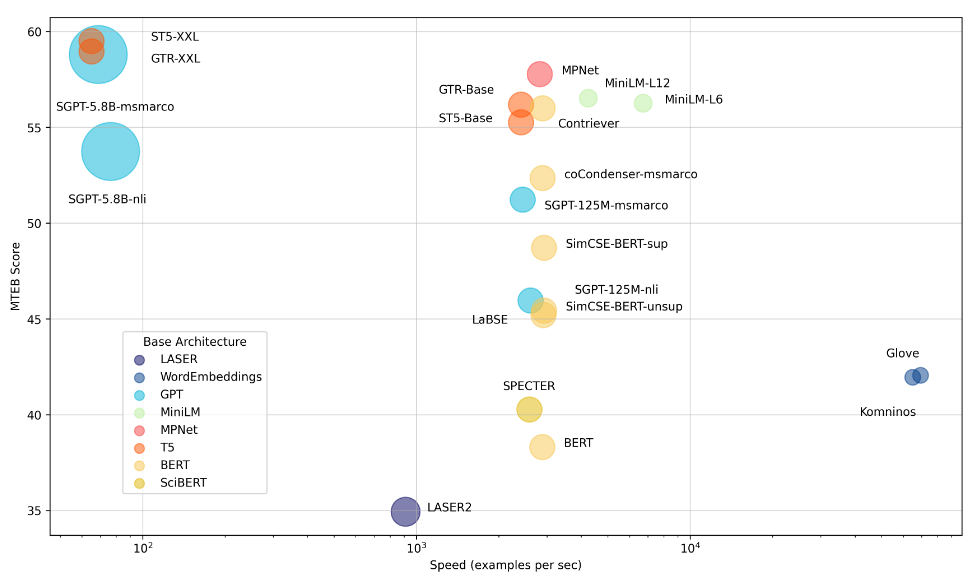
\includegraphics[width=\linewidth]{images/mteb-models.png}
    \caption{Сравнение точности, производительности и размеров моделей, приведенных в исследовании \cite{mteb}}
    \label{img:mteb_models}
\end{figure}

По результатам сравнения моделей на задаче кластеризации \cite{mteb}, лучших результатов с практически одинаковой точностью достигли следующие модели:
\begin{itemize}
    \item ST5-XXL;
    \item MPNet;
    \item GTR-XXL;
    \item MiniLM-L6
    \item ST5-XL.
\end{itemize}
TODO: лучше таблицей.

Несмотря на то, что модели ST5 и GTR имеют существенно больший размер и, соответственно, меньшую скорость работы, они незначительно опередели модели MPNet и MiniLM, которые практически в 50 раз меньше. Причиной этого может быть то, что MPNet и MiniLM дообучались на разнообразном датасете (для разных NLP-задач).

TODO: написать подробнее про классификацию алгоритмов кластеризации из \cite{no-patterns}.
Кратко:
\begin{itemize}
    \item Representative-based clustering (k-means и похожие);
    \item Иерархическая кластеризация (HAC);
    \item Density-based clustering (DBSCAN).
\end{itemize}

В работе \cite{deep-clustering-survey} приводится обзор применнеия методов глубокого обучения для снижения размерности пространства признаков, чтобы алгоритмы кластеризации лучше справлялись с большими объемами данных с большим количеством признаков. Но эта статья не про кластеризацию текста, а в целом про кластеризацию. TODO: написать.

В работе \cite{compare-text-clustering-sokolov} произведено сравнение следующих методов кластеризации текстовой информации: метод k-средних, алгоритм спектральной кластеризации, алгоритм агломеративной кластеризации и самоорганизующаяся карта Кохонена. В качестве данных использовалась коллекция новостей на русском языке. Для получения эмбедингов текста применялся алгоритм "мешок слов" ("bag of words"). В этой модели весь текст представлен одним вектором, хранящим информацию о количественном составе каждого слова в тексте. Недостатком данного подхода является отсутствие семантических связей между словами в тексте. В результате сравнения, алгоритмы показали достаточно близкую точность работы между собой, но, в среднем, самоорганизующиеся карты Кохонена оказались лучше других. Используемые алгоритмы сильно зависят от настройки гиперпараметров. Оптимальные параметры подбирались автоматически.

В работе \cite{method-text-clustering-andreev} дается обзор различных методов кластеризации, такие как: метод k-средних, suffix tree clustering, иерархические методы single link, complete link, group average, самоорганизующаяся карты Кохонена и сети ART (TODO: ???).
